\documentclass[11pt]{article}

\usepackage[letterpaper, margin=1in]{geometry}

\usepackage[spanish]{babel}
\usepackage[utf8]{inputenc}
\usepackage{multirow}
\usepackage{tabularx}
\usepackage{longtable}



%Figuras
\usepackage{graphicx, subfigure}
\usepackage[]{tikz}
\usepackage{pbox}

%Matemática
\usepackage{amsmath}
\usepackage{amssymb}

%Símbolos mate extra (alfabetos, etc.)
\usepackage{mathrsfs}


%Algoritmos
\usepackage{float}
\usepackage{algorithm}
\usepackage{algorithmicx}
\usepackage{algpseudocode}
\usepackage{listings}


\usepackage{color}
\usepackage{hyperref}

\usepackage{mdframed}
\usepackage{tcolorbox}
\usepackage{multicol}
\usepackage{booktabs}
\usepackage{tabulary}
\definecolor{darkblue}{rgb}{0 , 0.054 , 0.196}



\title{Reporte de proyecto corto}
\author{Pablo Alfaro Castro - B20162\\Carlos - B2}

\begin{document}

\maketitle
\hrule
\hrule
\tableofcontents
\hspace{5mm}
\hrule
\hrule


\section{Introducción}

El presente informe corresponde a el Laboratorio 0, el cual consistió en elaborar un programa "Sumador" en diversos lenguajes, ademas de programar un "Makefile" con diversas funciones y también se comento cada programa con la herramienta "Doxygen". Por ultimo se utilizo la herramienta "Git" para lograr subir el archivo a un repositorio.

\subsection{Objetivos}
El objetivo principal del laboratorio es aprender a manejar herramientas útiles para la programación como lo son Git, Make y Doxygen.



\section*{Código}

La figura \ref{fig:py} muestra el código escrito en el lenguaje Python, ademas muestra la forma en la que se comento con el formato de Deoxygen para generar los archivos buscados con ese método, sin embargo se presentaron algunas dificultades al momento de generar estos.

\begin{figure}[H]
\centering
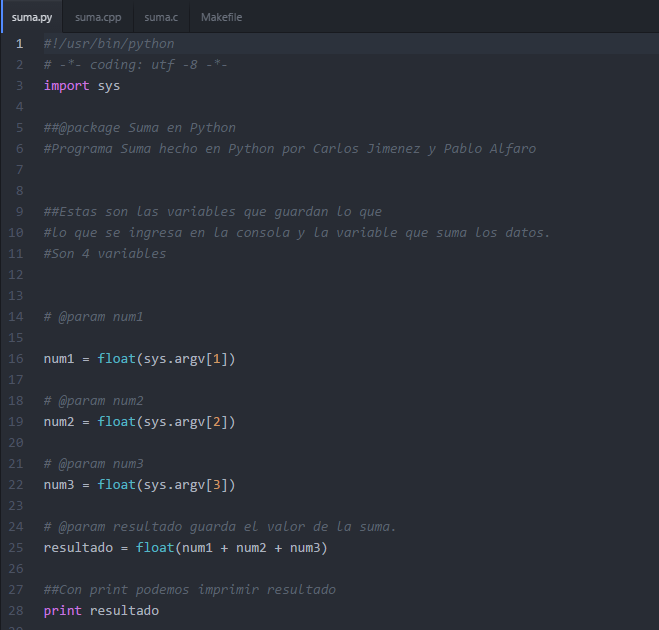
\includegraphics[scale=0.8]{img/py.png}
\caption{Código en Python}
\label{fig:py}
\end{figure}
\newpage

La figura \ref{fig:c} muestra el código escrito en el lenguaje C, ademas muestra la forma en la que se comento con el formato de Deoxygen para generar los archivos buscados con ese método, sin embargo se presentaron algunas dificultades al momento de generar estos.

\begin{figure}[H]
\centering
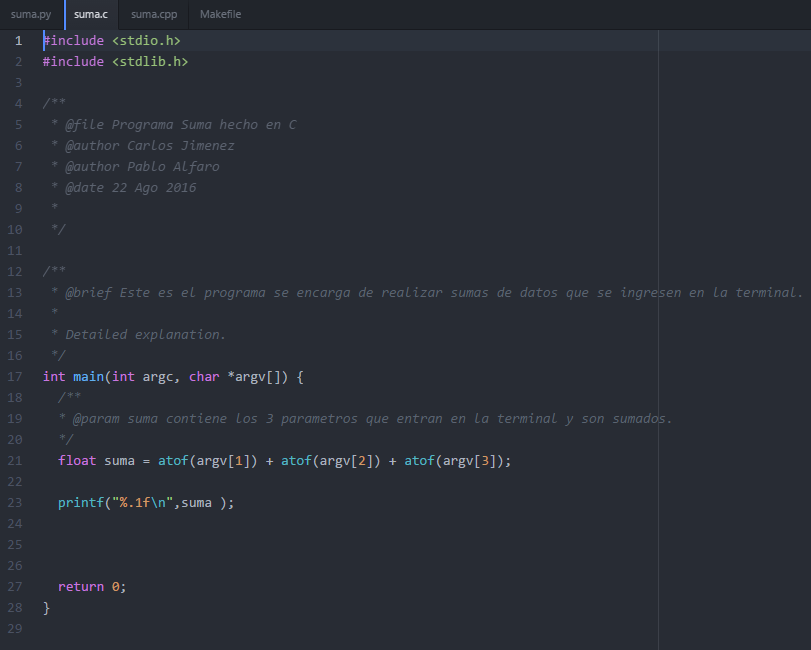
\includegraphics[scale=0.8]{img/c.png}
\caption{Código en C}
\label{fig:c}
\end{figure}
\newpage

La figura \ref{fig:cp} muestra el código escrito en el lenguaje C++, ademas muestra la forma en la que se comento con el formato de Deoxygen para generar los archivos buscados con ese método, sin embargo se presentaron algunas dificultades al momento de generar estos.

\begin{figure}[H]
\centering
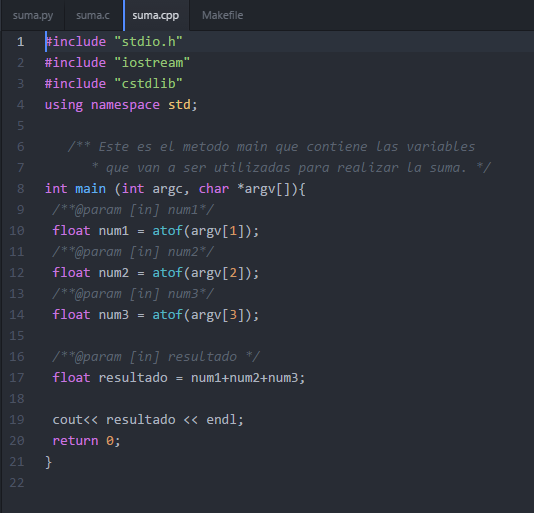
\includegraphics[scale=0.8]{img/cp.png}
\caption{Código en C++}
\label{fig:cp}
\end{figure}
\newpage

Por ultimo se implemento el Mekefile el cual fue completamente funcional y se programo de la manera que cumplió los tres objetivos pedidos que son compilar, borrar y ejecutar, como se ve en la figura \ref{fig:mk}.

\begin{figure}[H]
\centering
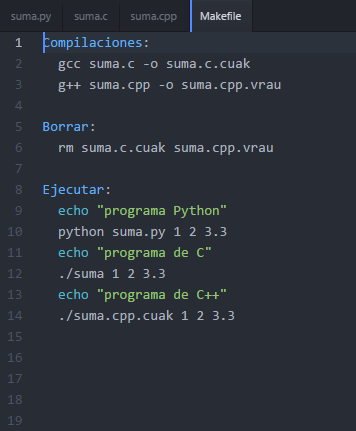
\includegraphics[scale=0.8]{img/mk.png}
\caption{Código del Makefile}
\label{fig:mk}
\end{figure}
\newpage

\section*{GitHub}

El primer paso en el tutorial correspondió a inicializar un repositorio, que se logro con el comando que se muestra:

\begin{figure}[H]
\centering
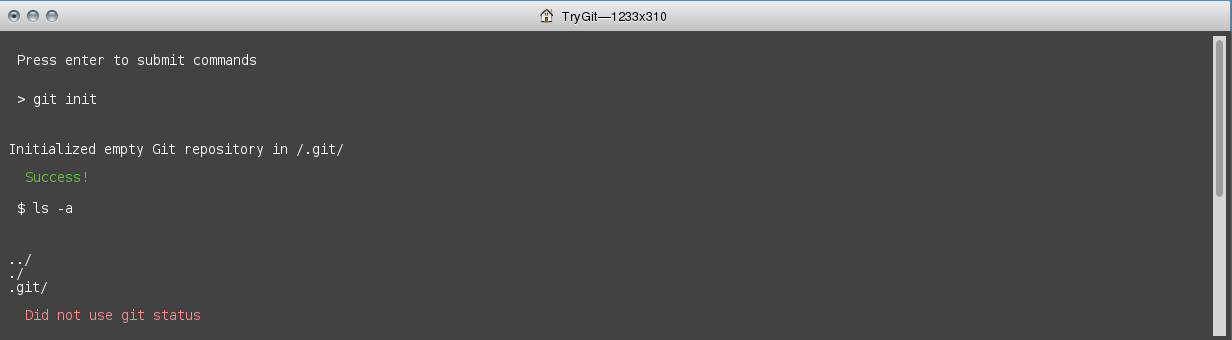
\includegraphics[scale=0.8]{img/1.png}
\caption{Paso 1}
\label{fig:1}
\end{figure}

Lo siguiente fue verificar el estado del repositorio:

\begin{figure}[H]
\centering
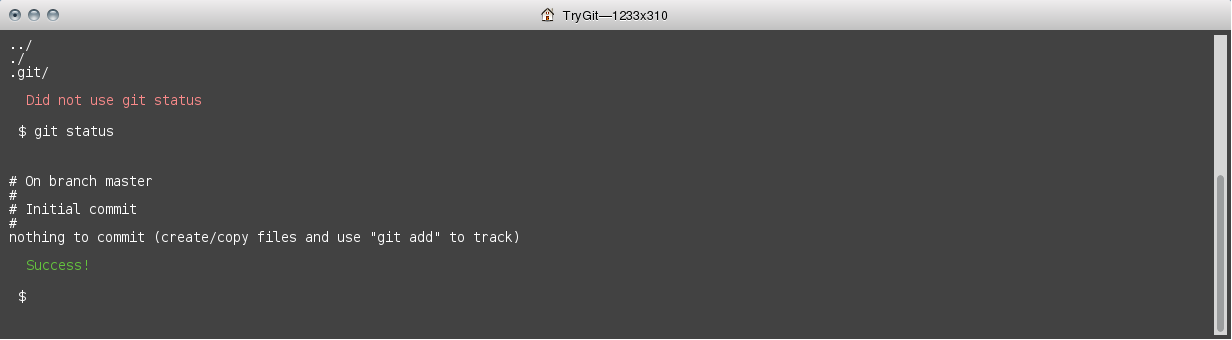
\includegraphics[scale=0.8]{img/2.png}
\caption{Paso 2}
\label{fig:2}
\end{figure}



\begin{figure}[H]
\centering
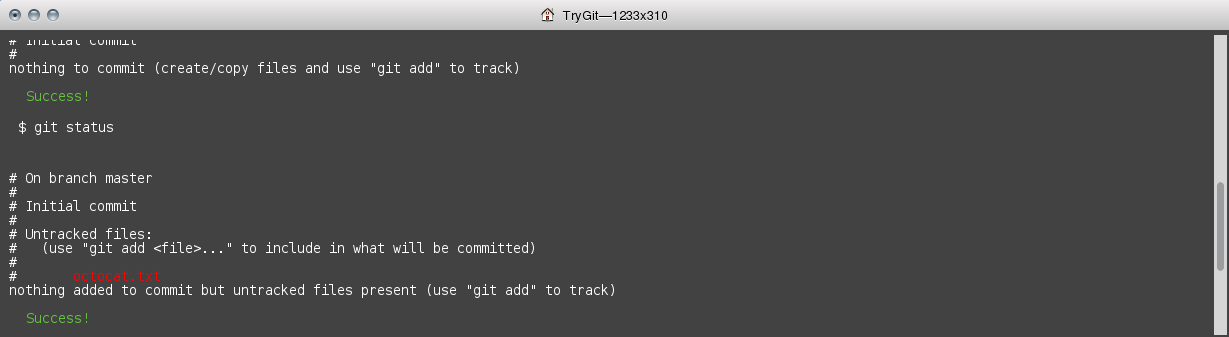
\includegraphics[scale=0.8]{img/3.png}
\caption{Paso 3}
\label{fig:3}
\end{figure}

El siguiente paso fue agregar un archivo al repositorio:


\begin{figure}[H]
\centering
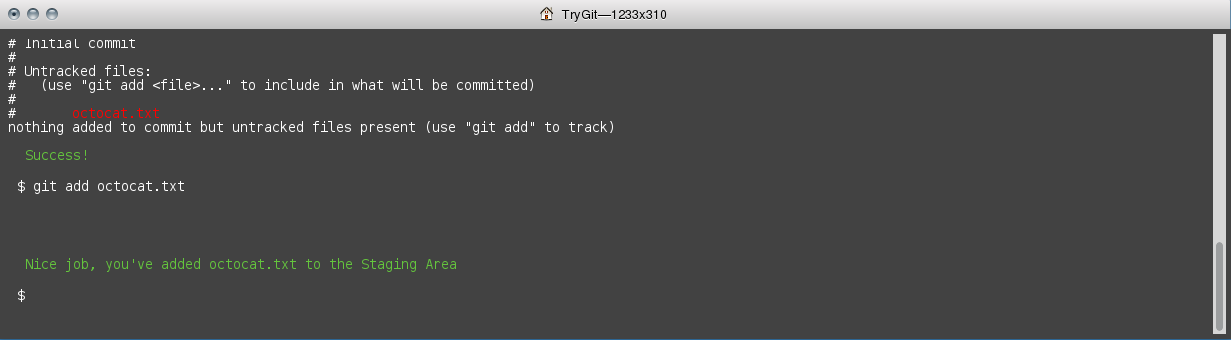
\includegraphics[scale=0.8]{img/4.png}
\caption{Paso 4}
\label{fig:4}
\end{figure}
Ahora se verifico de nuevo el estado del repositorio:



\begin{figure}[H]
\centering
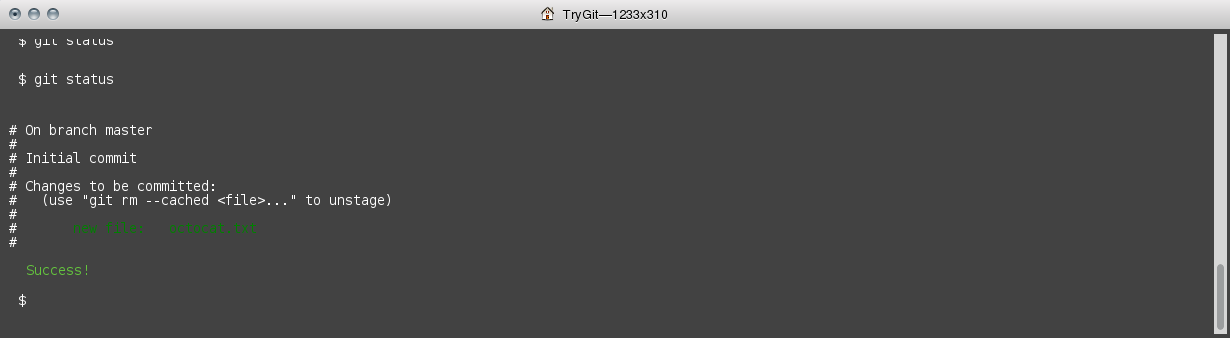
\includegraphics[scale=0.8]{img/5.png}
\caption{Paso 5}
\label{fig:5}
\end{figure}

Se realizo un commit para lograr salvar los cambios:


\begin{figure}[H]
\centering
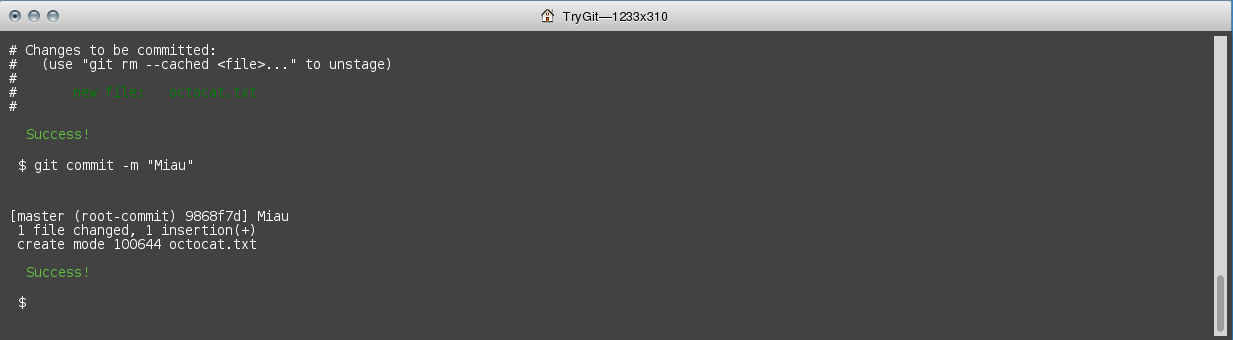
\includegraphics[scale=0.8]{img/6.png}
\caption{Paso 6}
\label{fig:6}
\end{figure}

se realizo un commit para todos los cambios en el repositorio:

\begin{figure}[H]
\centering
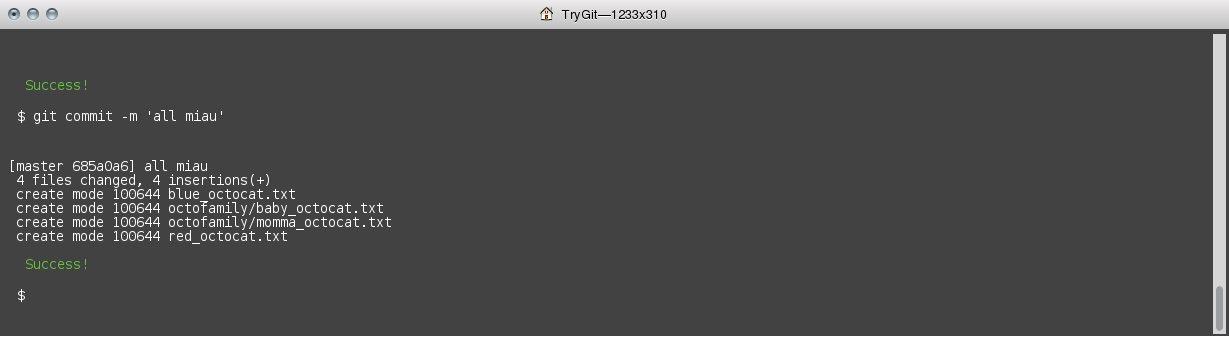
\includegraphics[scale=0.8]{img/7.png}
\caption{Paso 7}
\label{fig:7}
\end{figure}

En este paso se realizo una verificación de cambios:

\begin{figure}[H]
\centering
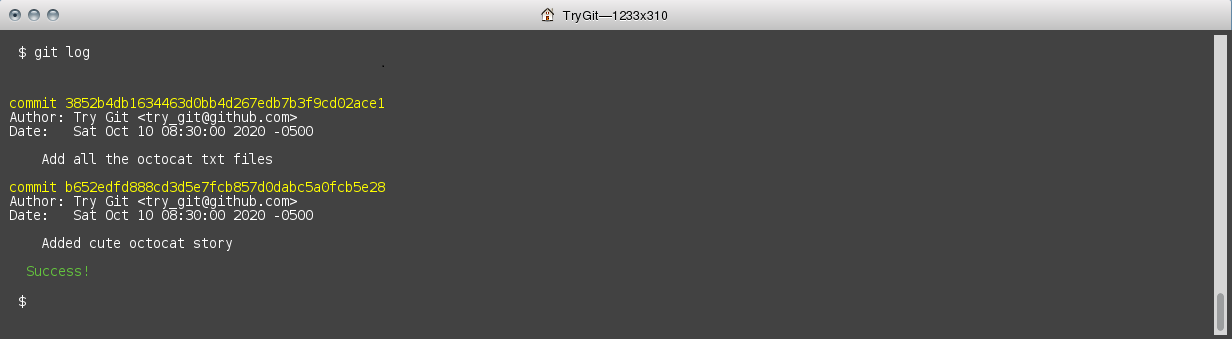
\includegraphics[scale=0.8]{img/8.png}
\caption{Paso 8}
\label{fig:8}
\end{figure}

El siguiente paso fue tomar un repositorio mediante una dirección web:

\begin{figure}[H]
\centering
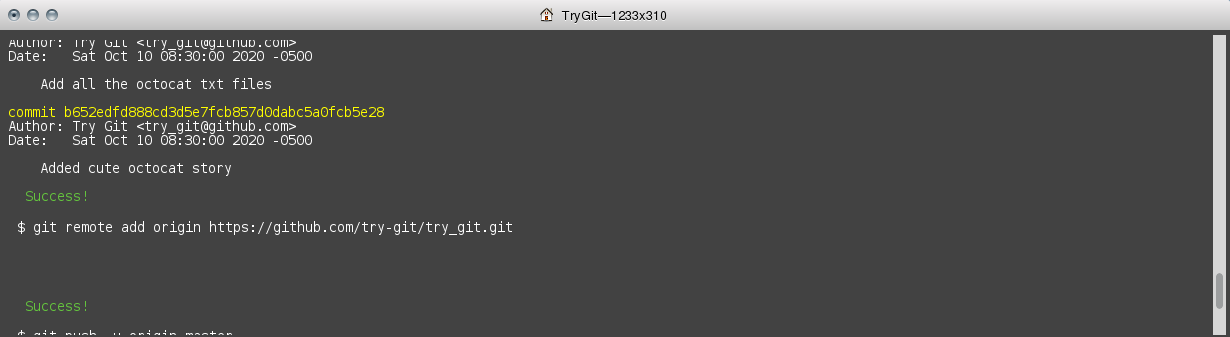
\includegraphics[scale=0.8]{img/9.png}
\caption{Paso 9}
\label{fig:9}
\end{figure}

Se utilizo la herramienta pull para analizar los cambios:

\begin{figure}[H]
\centering
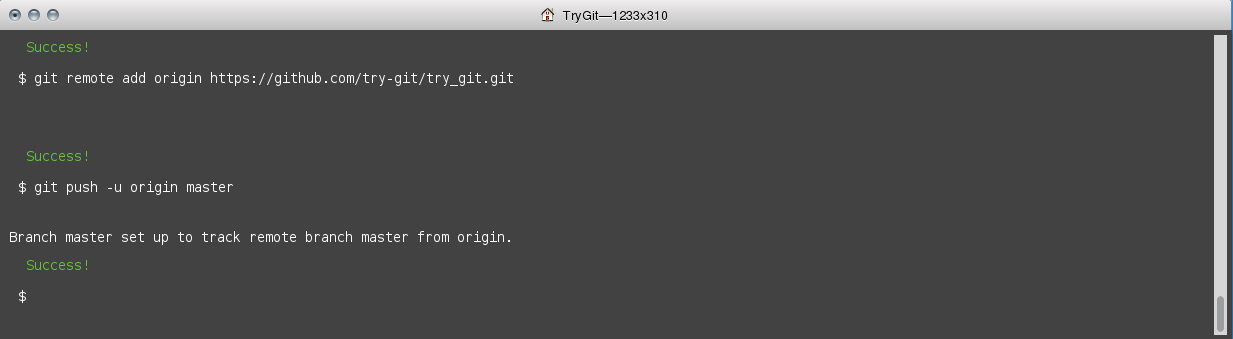
\includegraphics[scale=0.8]{img/10.png}
\caption{Paso 10}
\label{fig:10}
\end{figure}

\begin{figure}[H]
\centering
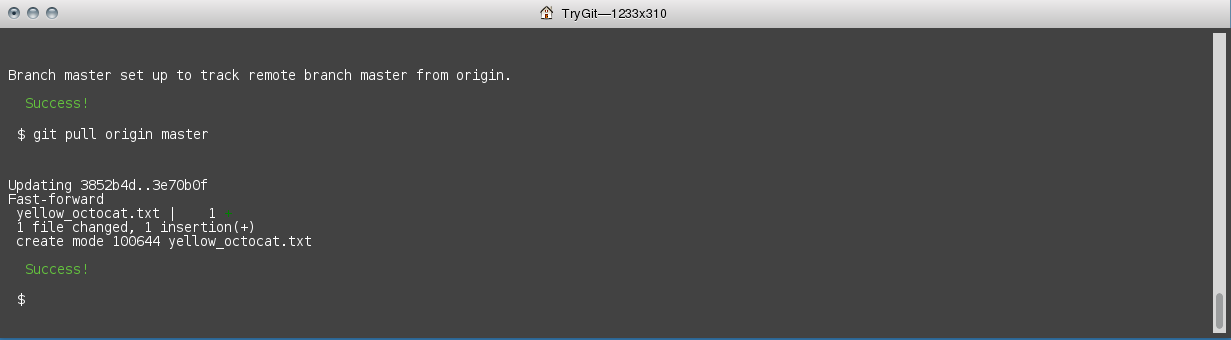
\includegraphics[scale=0.8]{img/11.png}
\caption{Paso 11}
\label{fig:11}
\end{figure}



\begin{figure}[H]
\centering
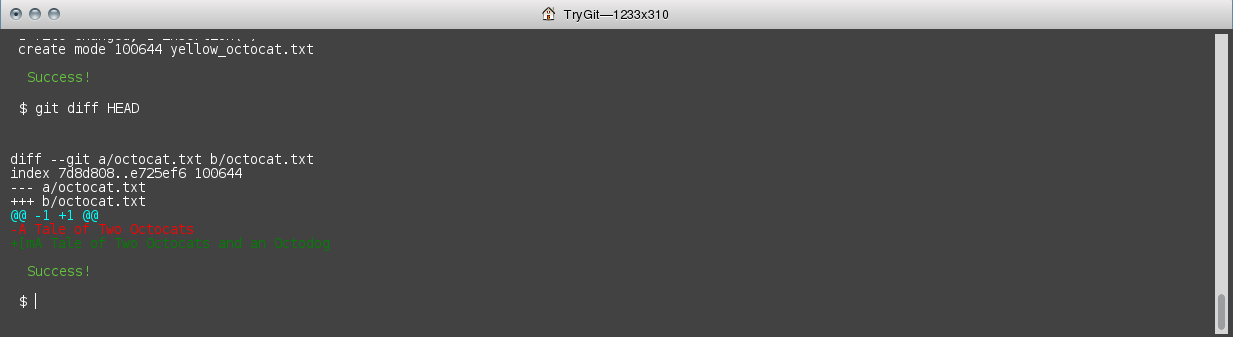
\includegraphics[scale=0.8]{img/12.png}
\caption{Paso 12}
\label{fig:12}
\end{figure}

Se añadieron algunas carpetas extra al repositorio:

\begin{figure}[H]
\centering
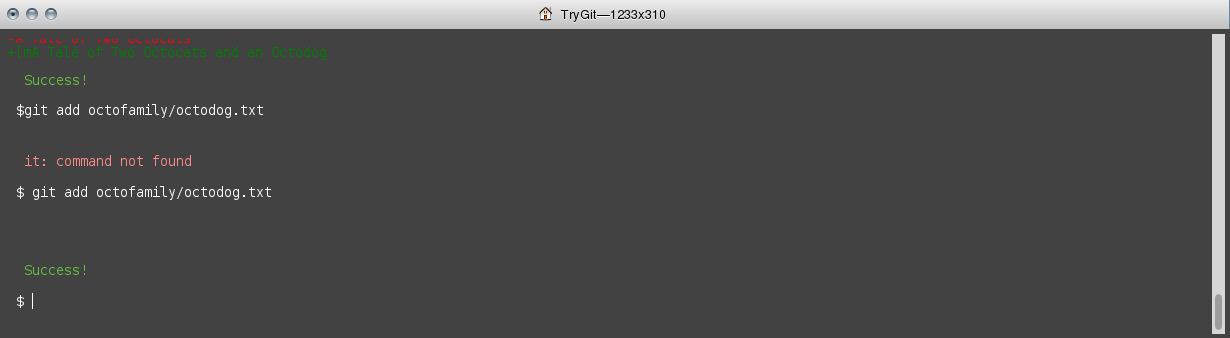
\includegraphics[scale=0.8]{img/13.png}
\caption{Paso 13}
\label{fig:13}
\end{figure}

Se ejecuto el comando diff para ver el ultimo cambio que se hizo:

\begin{figure}[H]
\centering
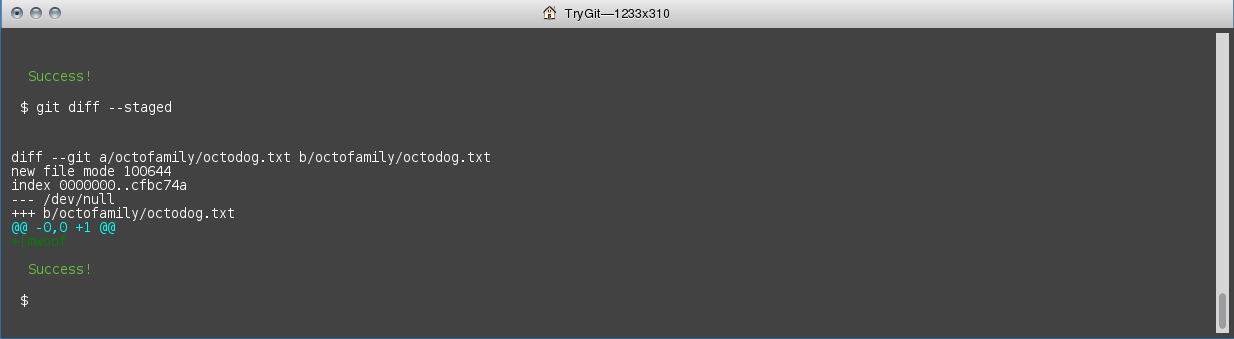
\includegraphics[scale=0.8]{img/14.png}
\caption{Paso 14}
\label{fig:14}
\end{figure}

Ahora se reseteo para remover le directorio anteriormente agregado:


\begin{figure}[H]
\centering
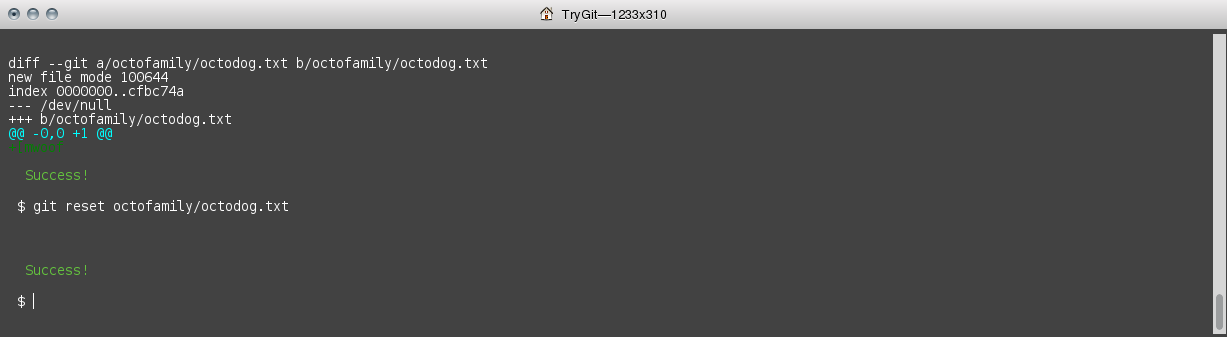
\includegraphics[scale=0.8]{img/15.png}
\caption{Paso 15}
\label{fig:15}
\end{figure}

Se realizo el checkout sobre el archivo que seguimos:	

\begin{figure}[H]
\centering
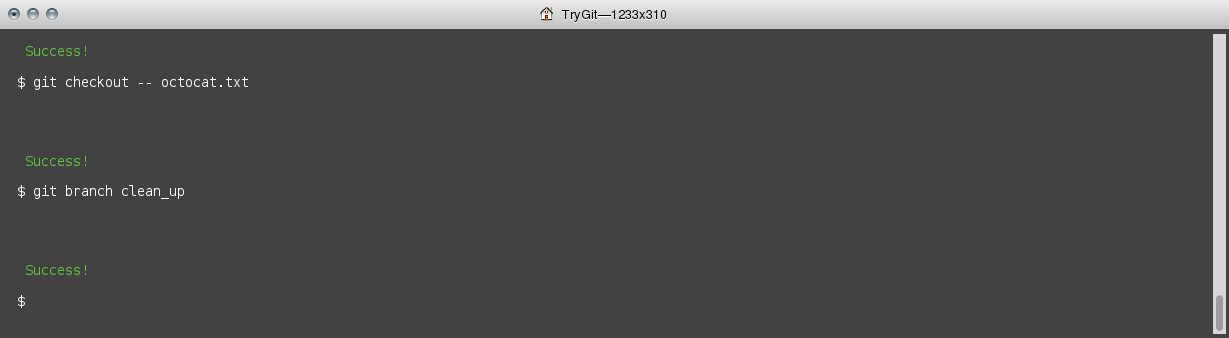
\includegraphics[scale=0.8]{img/16.png}
\caption{Paso 16}
\label{fig:16}
\end{figure}

\begin{figure}[H]
\centering
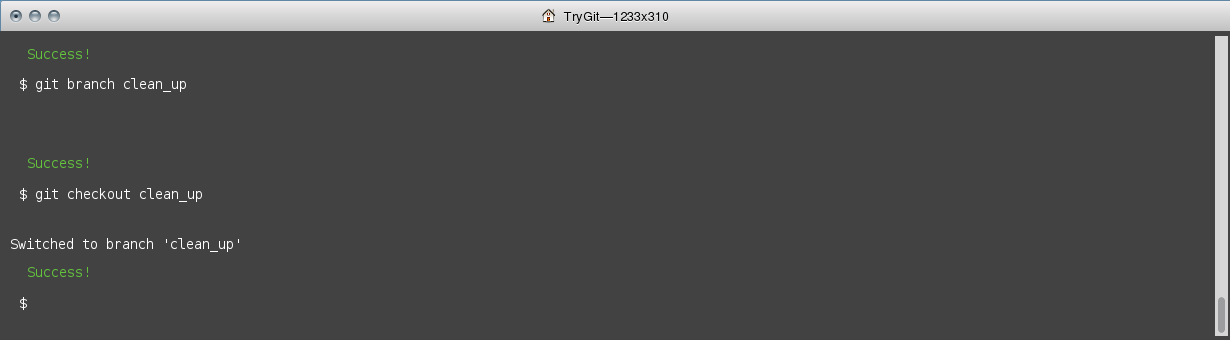
\includegraphics[scale=0.8]{img/17.png}
\caption{Paso 17}
\label{fig:17}
\end{figure}

Con git rm se eliminaron los archivos no solo del disco sino tambien del repositorio:

\begin{figure}[H]
\centering
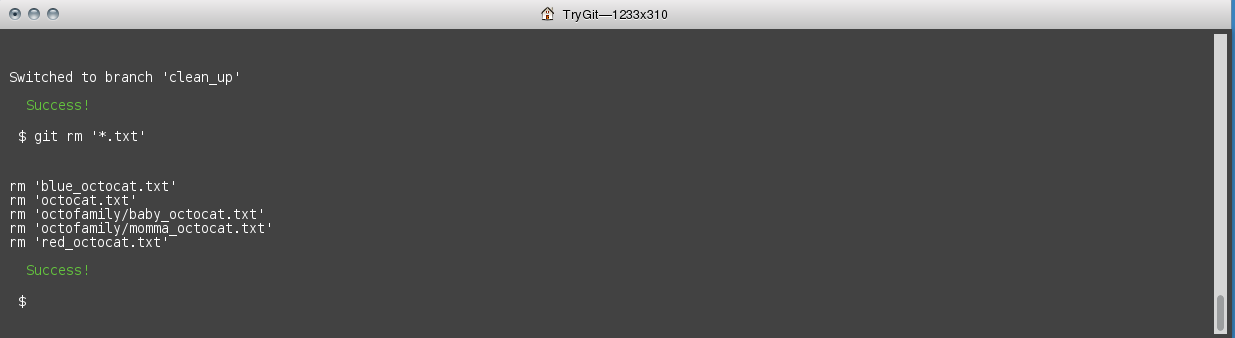
\includegraphics[scale=0.8]{img/18.png}
\caption{Paso 18}
\label{fig:18}
\end{figure}

Se realizo un commit para guardar los cambios:

\begin{figure}[H]
\centering
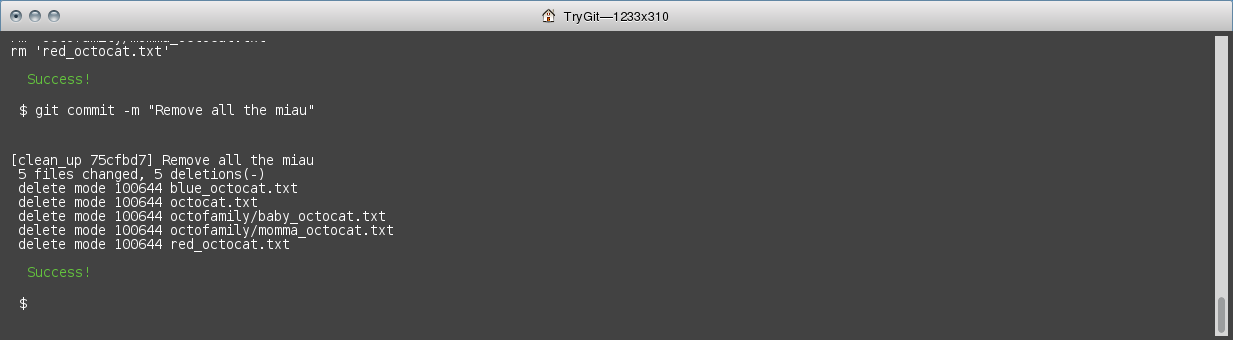
\includegraphics[scale=0.8]{img/19.png}
\caption{Paso 19}
\label{fig:19}
\end{figure}

Se procedió a realizar algunos comandos intermedios:

\begin{figure}[H]
\centering
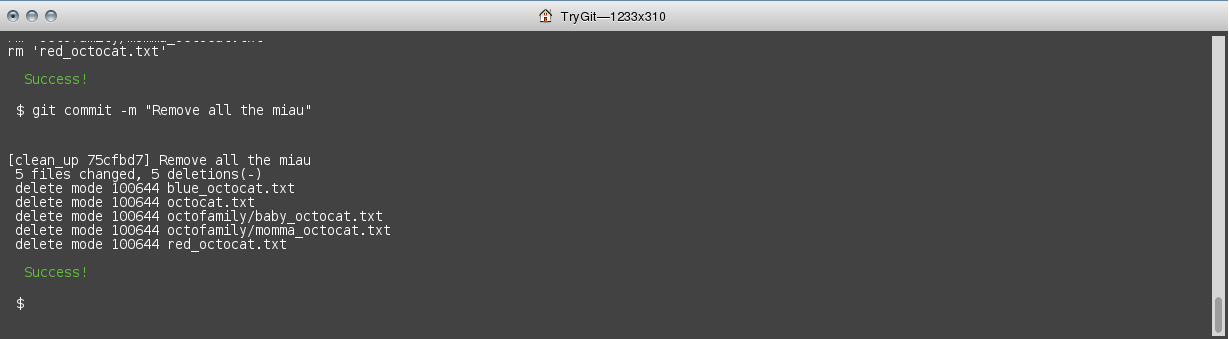
\includegraphics[scale=0.8]{img/20.png}
\caption{Paso 20}
\label{fig:20}
\end{figure}

\begin{figure}[H]
\centering
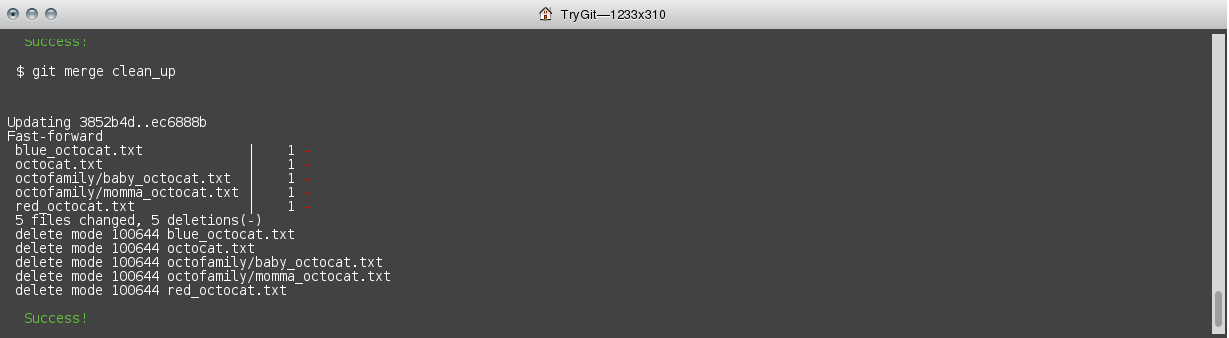
\includegraphics[scale=0.8]{img/21.png}
\caption{Paso 21}
\label{fig:21}
\end{figure}
Por ultimo se realizo un push final:
\begin{figure}[H]
\centering
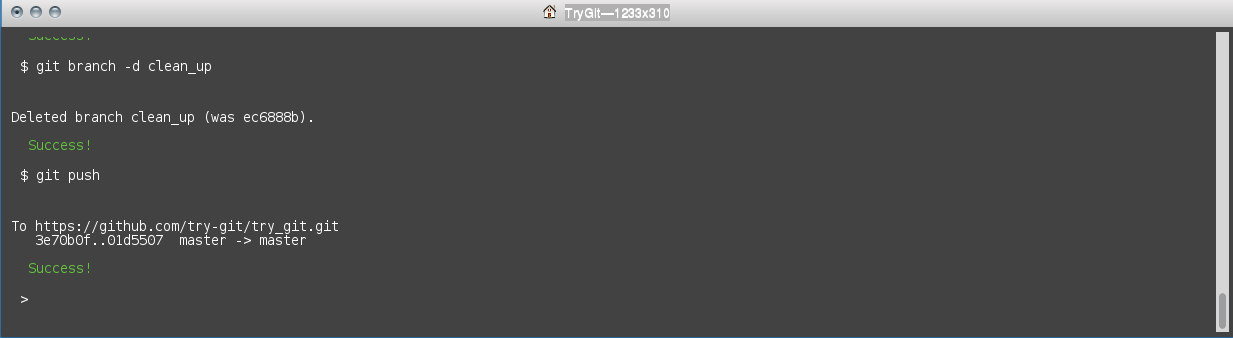
\includegraphics[scale=0.8]{img/22.png}
\caption{Paso 22}
\label{fig:22}
\end{figure}

\section{Conclusiones}

\begin{itemize}
\item Se pudo aprender lo básico en cuanto al manejo de versiones, compilación y documentación.
\end{itemize}










\end{document}
